\documentclass[{../../master}]{subfiles}
\graphicspath{{../../}}  % 個別コンパイル時の画像パスを解決する

\begin{document}

\section{RPLiDAR A2を利用する}

\subsection{製品の概要}

RPLiDAR A2は,SLAMTEC社から発売されている安価な360°計測可能なLiDARセンサです.

\begin{figure}[ht]
  \centering
  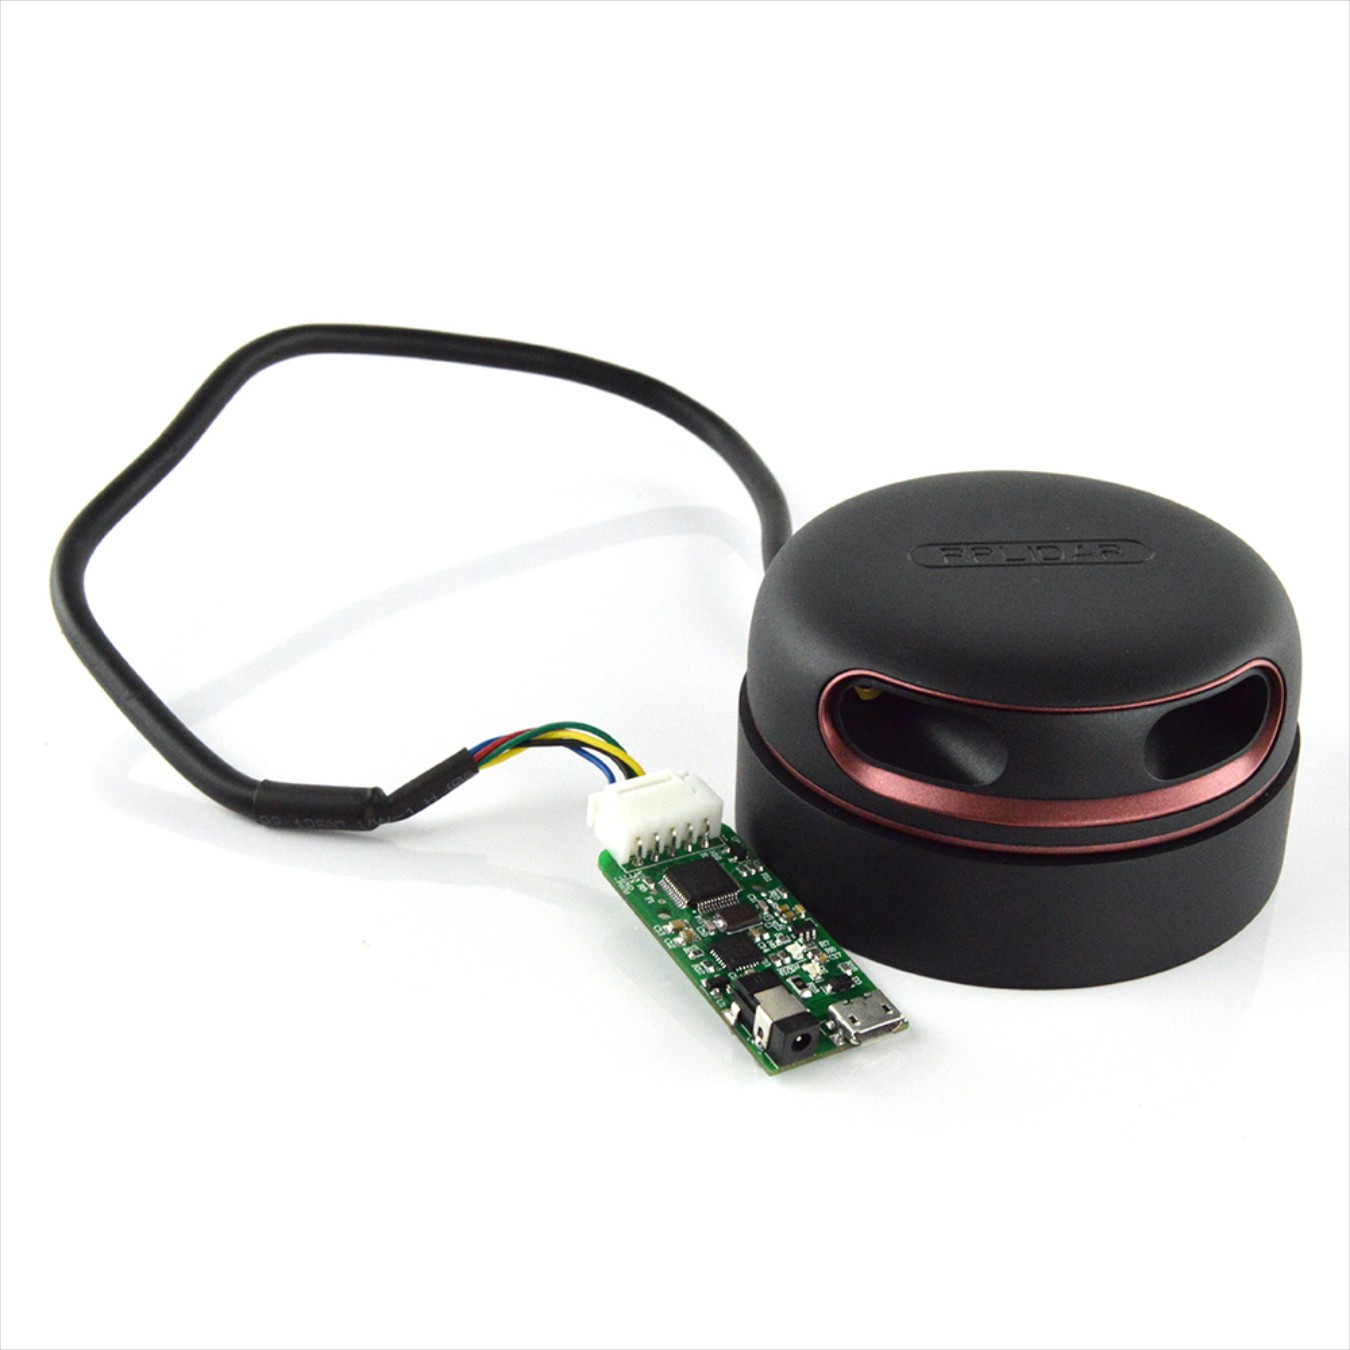
\includegraphics[height=50truemm]{images/rplidar_a2.jpg}
  \caption{SLAMTEC RPLiDAR A2}
\end{figure}

RPLiDARシリーズのROSドライバは既に用意されているため\footnote{\url{http://wiki.ros.org/rplidar}},購入後すぐに利用することができます.

\subsection{launchファイルの用意}
\label{sec:prepare_rplidar_launch}

RPLiDAR A2を起動するためのlaunchファイルを作成します.
\textsf{adamr2\_bringup}パッケージの\textsf{launch/}ディレクトリに,\textsf{rplidar\_a2.launch}という名前のファイルを作成し,コード\ref{code:rplidar_a2_launch}のように記述します.

\begin{lstlisting}[language=XML, label=code:rplidar_a2_launch, caption=\textsf{rplidar\_a2.launch}]
<launch>
  <arg name="device"   default="/dev/ttyUSB0"/>
  <arg name="baudrate" default="115200"/>
  <arg name="frame_id" default="lidar_link"/>
  <arg name="inverted" default="false"/>
  <arg name="angle_compensate" default="true"/>

  <group ns="/adamr2">
    <node name="rplidarNode" pkg="rplidar_ros" type="rplidarNode" output="screen">
      <param name="serial_port"      type="string" value="$(arg device)"/>
      <param name="serial_baudrate"  type="int"    value="$(arg baudrate)"/>
      <param name="frame_id"         type="string" value="$(arg frame_id)"/>
      <param name="inverted"         type="bool"   value="$(arg inverted)"/>
      <param name="angle_compensate" type="bool"   value="$(arg angle_compensate)"/>
    </node>
  </group>
</launch>
\end{lstlisting}

RPLiDARのROSドライバノードである\textsf{rplidarNode}は,以下の6つのパラメータを取ります.

\begin{enumerate}
  \item \textsf{serial\_port}
  \item \textsf{serial\_baudrate}
  \item \textsf{frame\_id}
  \item \textsf{inverted}
  \item \textsf{angle\_compensate}
  \item \textsf{scam\_mode}
\end{enumerate}

\textsf{serial\_port}はRPLiDARのデバイスファイルを指定します.
RPLiDAR A2のデバイスファイルは,他にUSBデバイスを繋いでいなければ「\textsf{/dev/ttyUSB0}」になります.
\textsf{serial\_baudrate}はシリアル通信のボーレートです.RPLiDAR A2ならばボーレートは115200固定です.
\textsf{frame\_id}はLiDARのTFフレーム名を指定します.
\ref{sec:add_lidar_link}でURDFを記述した際に,「\textsf{lidar\_link}」という名前を付けていたので,ここではそれを指定します.

また,ノードに名前空間を設定しています.
名前空間の設定は必須ではありませんが,\footnote{複数台のロボットを制御したりしないのであれば,むしろデフォルトのままの方が混乱が起きにくいです.}
ここでは\textsf{scan}メッセージにも名前空間を指定することにします.

\subsection{RPLiDARを使ってみる}

早速作成したlaunchファイルを実行して,RPLiDARを使ってみましょう.
RPLiDARをPCに接続して,launchファイルを実行します.

\begin{lstlisting}[language=sh, caption=Launch \textsf{rplidar\_a2.launch}]
roslaunch adamr2_bringup rplidar_a2.launch
\end{lstlisting}

無事にノードが起動したら,\textsf{rviz}を起動してセンサデータを確認してみましょう.
固定フレームに「\textsf{lidar\_link}」を指定します.
TFが配信されていないのでプルダウンメニューには表示されません.
名前を直接入力しましょう.
次に左下の「Add」ボタンから「LaserScan」を追加し,トピック名に「\textsf{adamr2/scan}」を指定します.
センサデータが見えるようになればOKです.

\end{document}